\section{Resultados}
\subsection{Densidade do líquido}
Definindo a linha paralela à separação da fase de água com a fase do líquido
misterioso como ponto de altura \(h = 0\), determinamos a altura em que a
água fica exposta ao ar como \(h_w = \qty{0,123}{m}\) e a altura na qual o
líquido misterioso fica exposto ao ar como \(h_l = \qty{0,153}{m}\). 

\subsection{Manômetros}
Os valores obtidos estão sintetizados na \cref{tab_man}.

\begin{table}[H]
    \centering
    \begin{tabular}{c | c | c}
        \hline
        \textbf{E. Livre (cm \(\pm 0,5\))} & \textbf{E. Atm (cm\(\pm 0,5\))} & \textbf{E. Recip (cm \(\pm0,5\))}\\
        \hline
        0,0 & 12,2 & 12,2\\
        \hline
        5,0 & 14,5 & 11,1\\
        \hline
        10,0 & 16,2 & 9,0\\
        \hline
    \end{tabular}
    \caption{Valores mensurados com o manômetro de tubo aberto}
    \label{tab_man}
\end{table}

\subsection{Discos de Magdeburg}
Durante a realização do experimento, não foi possível separar os discos. Além
disso, não foi observada nenhuma deformação significativa, isto é, não foi
observada qualquer tendência de movimento. 

\subsection{Frasco com membrana}
Após a retirada da interface plástica o líquido se manteve dentro do frasco. Em
seguida, na análise da inclinação com o software Traker, obtemos a \cref{copo.png}. Veja
\begin{figure}[H]
    \centering
    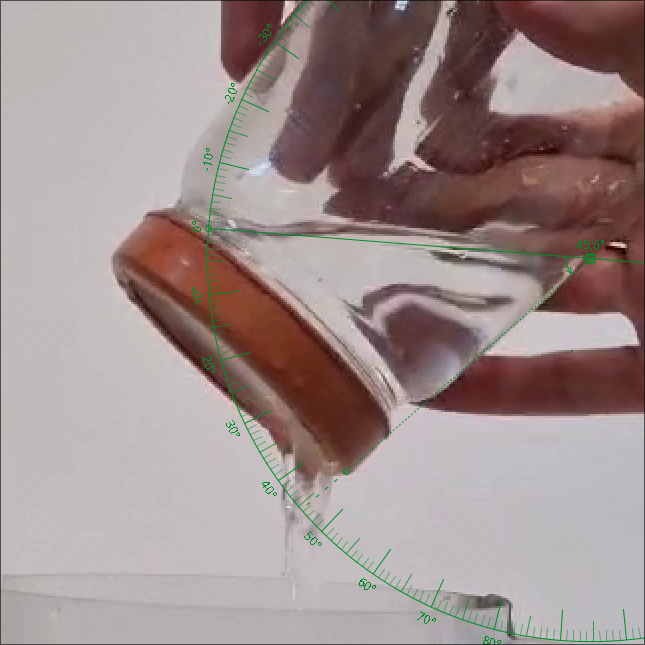
\includegraphics[width=.35\linewidth]{fig/copo.png}
    \caption{Ângulo de inclinação do copo para equilíbrio de pressões}
    \label{copo.png}
\end{figure}

Note a inclinação do frasco em relação ao nível da água, em torno de \( 45,6 \)°
.

